\subsection{Combined Datasets}
\label{sub:dataset_cross_val}

After finding consistent results between classifiers for each dataset (Motion Sense and MobiAct), we performed a quick test of how similar the datasets are---we na\"ively attempted to use a classifier trained on Motion Sense to predict activity in MobiAct and vice versa. We used only used the accelerometer data, in line with our previous test classifiers. The Motion Sense dataset had removed the acceleration due to gravity from the accelerometer data while the MobiAct did not. In order to have consistent data, we added back in the acceleration due to gravity into the Motion Sense data. After this, we decided to combine the datasets and run our classifiers. 

To make as fair a comparison as possible, we only attempted to predict entries that were labeled as an activity that appeared in both datasets. We only evaluated ourselves on the following activities: walking, jogging, sitting, standing, walking upstairs, and walking downstairs. After some deliberation, we decided to increase the feature vector length to 5.12 seconds (i.e.\ 256 samples), in order to better capture the periodicity of the signals. A summary of our results for the 128- and 256-dimensional feature vectors are given in Tables~\ref{tab:128naive}~and~\ref{tab:256naive} below.

% \begin{table}[H]
% \centering
% \caption{Na\"ive Cross Dataset Prediction Accuracy}
% \begin{tabular}{lccl}
% \toprule
% \multicolumn{1}{l}{\textbf{Test Dataset}} & \multicolumn{1}{c}{\textbf{SVC}} & \multicolumn{1}{c}{\textbf{k-NN}} & \multicolumn{1}{c}{\textbf{Trees}}  \\ \midrule
% \textbf{Motion Sense} &  34.3\% & 34.6\% & 36.8\%     \\
% \textbf{UCI--HAR}      & 32.2\% & 20.0\% & 39.9\% \\
% \bottomrule
% \end{tabular}
% \end{table}

\begin{table}[H]
\centering
\caption{Cross Dataset Accuracy, 128 Feature Length}
\begin{tabular}{lcl}
\toprule
\multicolumn{1}{l}{\textbf{Test Dataset}} & \multicolumn{1}{c}{\textbf{k-NN}} & \multicolumn{1}{c}{\textbf{Trees}}  \\ \midrule
\textsc{MotionSense} & 39.4\% & 66.5\%  \\
\textsc{MobiAct}     & 42.9\% & 66.7\%  \\
\bottomrule
\end{tabular}
\label{tab:128naive}
\end{table}




\begin{table}[H]
\centering
\caption{Cross Dataset Accuracy, 256 Feature Length}
\begin{tabular}{lcl}
\toprule
\multicolumn{1}{l}{\textbf{Test Dataset}} & \multicolumn{1}{c}{\textbf{k-NN}} & \multicolumn{1}{c}{\textbf{Trees}}  \\ \midrule
\textsc{MotionSense}	& 36.8\%	& 68.6\% \\ 
\textsc{MobiAct}	&  44.3\%	& 77.0\% \\
\bottomrule
\end{tabular}
\label{tab:256naive}
\end{table}

The na\"ive approach was surprisingly accurate, after carefully taking into account the difference between them in preprocessing. Unfortunately, our approach for utilizing orientation data and principle component analysis to improve data alignment between datasets worsened the results.

\subsection{Data Orientation Processing}
\label{sub:rotating}

As shown in Figure \ref{fig:motionSense_sitting_comp}, we tried to devise a method to account for variation in the phone's orientation across datasets. The reported acceleration data is taken in the body frame of the phone. As a result, the x,y, and z acceleration axes shift when one moves, and are different depending on how one holds the phone. The MobiAct and Motion Sense datasets both contain information about the phone's orientation in the form of pitch, roll, and yaw. So, we created a rotation matrix based on the pitch, row, and yaw measurements. The rotation matrix tells us how the phone was rotated relatively to its initial position, which is intrinsic to each phone. To transform the acceleration vectors to be in the initial phone position, regardless of orientation, we need to rotate each of the acceleration vectors back to their initial positions, based on the orientation measurements. Thus, we need to use the inverse of the rotation matrix.

For simplicity, the initial rotation matrix ($R_q$), representing the current phone orientation, and acceleration vectors were represented as quaternions.

\begin{equation}
\label{eqn: quaternion_orientation}
    q = a + b\mathbf{i} + c\mathbf{j} + d\mathbf{k} = \mqty[
\cos (\phi /2) \cos (\theta /2) \cos (\psi /2) +  \sin (\phi /2) \sin (\theta /2) \sin (\psi /2) \\
\sin (\phi /2) \cos (\theta /2) \cos (\psi /2) -  \cos (\phi /2) \sin (\theta /2) \sin (\psi /2) \\
\cos (\phi /2) \sin (\theta /2) \cos (\psi /2) +  \sin (\phi /2) \cos (\theta /2) \sin (\psi /2) \\
\cos (\phi /2) \cos (\theta /2) \sin (\psi /2) -  \sin (\phi /2) \sin (\theta /2) \cos (\psi /2) ]
\end{equation}
where $\theta$, $\phi$, and $\psi$ correspond to the Euler angles representing the phone's roll, pitch, and yaw. Similarly, we have a quaternion representing the acceleration vector as measured by the accelerometer, 
\begin{equation}
\label{eqn:quaternion_acceleration}
    p = a' + b'\mathbf{i} + c'\mathbf{j} + d'\mathbf{k} = \mqty[0, a_x, a_y, a_z]^T
\end{equation}
where $(a_x, a_y, a_z)$ correspond to the tri-axial acceleration components.

The rotation of  acceleration by orientation can be done with quaternions as shown in Eqn.~(\ref{eqn:quaternion_rotation}) below
\begin{equation}
\label{eqn:quaternion_rotation}
    R_q(p) = q \odot p \odot q^{*},
\end{equation}
where $\odot$ represents the Hamilton Product and $^{*}$ represents the conjugate of the quaternion.

The inversion of the rotation matrix ($R_q^{-1}$) is equivalent to the conjugate of the corresponding quaternion ($q^{*}$).

\begin{figure}[ht]
  \centering
  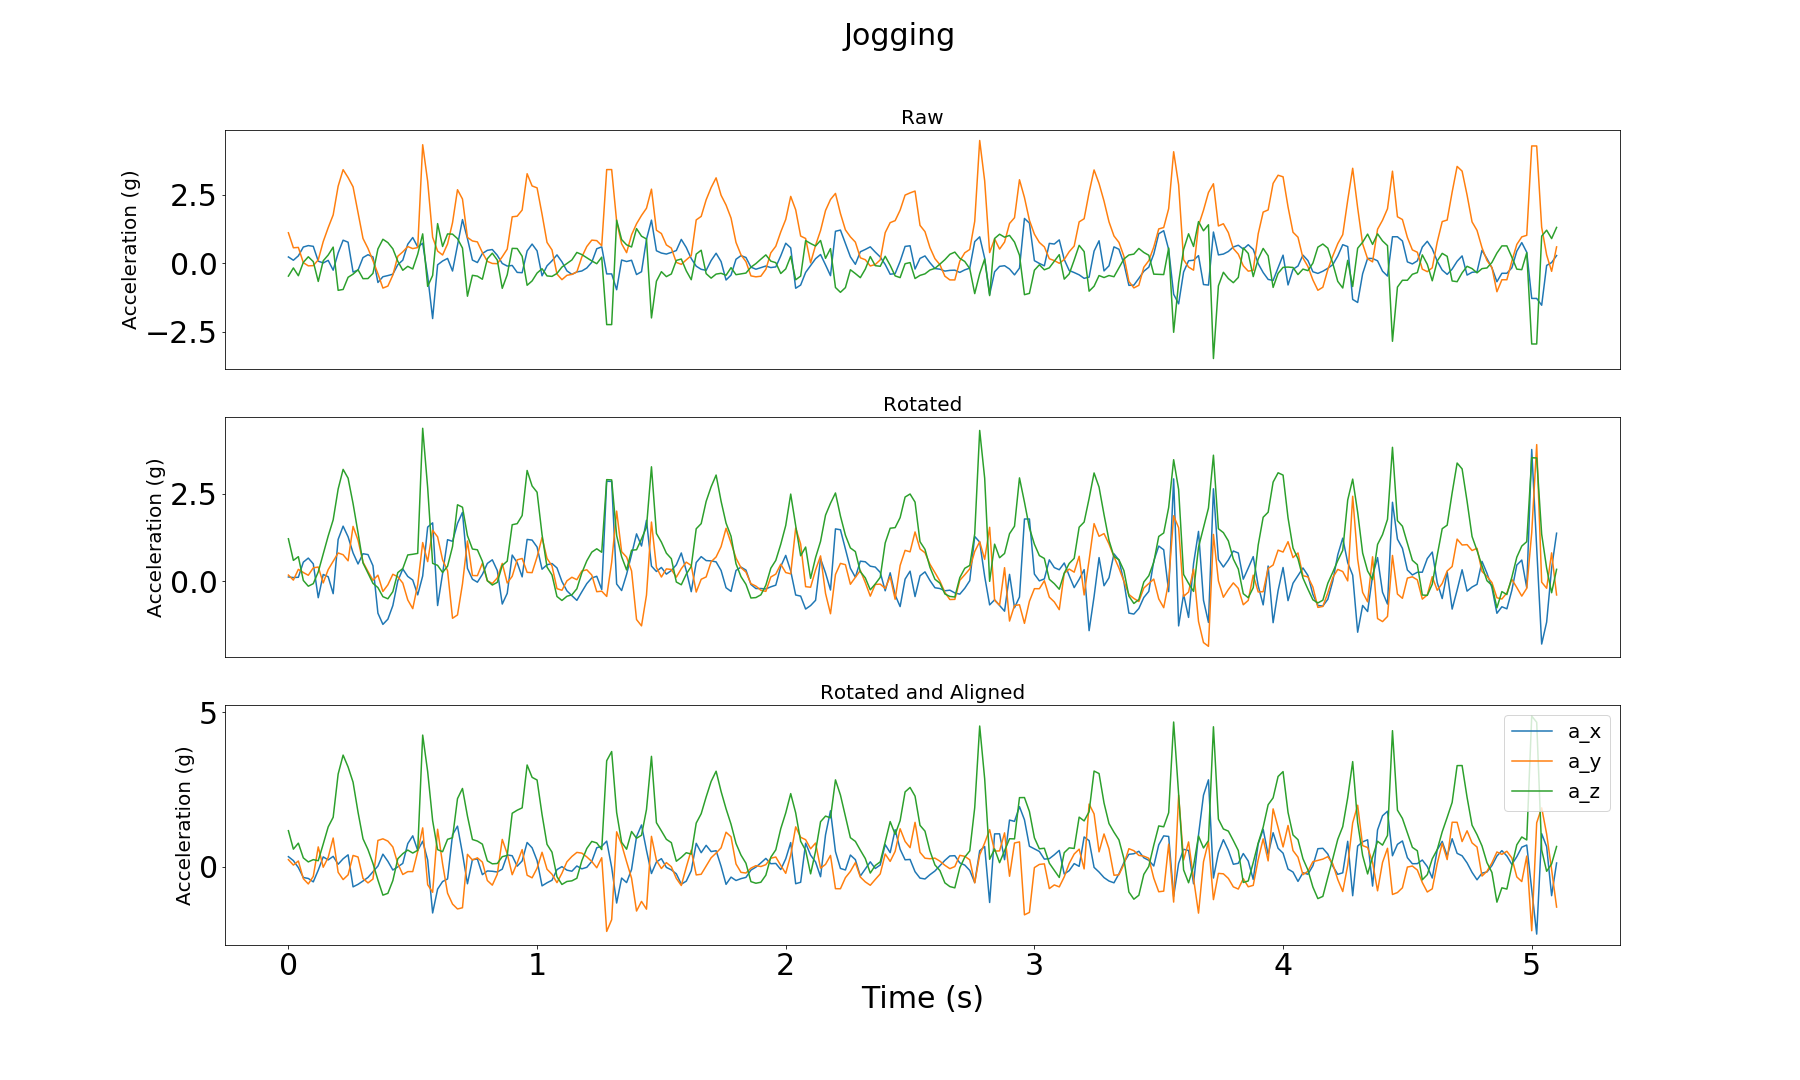
\includegraphics[width=1 \textwidth]{images/comparisons/jogIncrementalRotation.png}
    \caption{The orientation pre-processing initially utilizes the yaw, pitch, and roll angles to rotate the acceleration data back to the phone's initial position. PCA is then used to find the axis with the most variation, which is then projected onto the $z$-axis.}
     \label{fig:rotationAlignmentComp}
\end{figure}


\begin{figure}[ht]
  \centering
  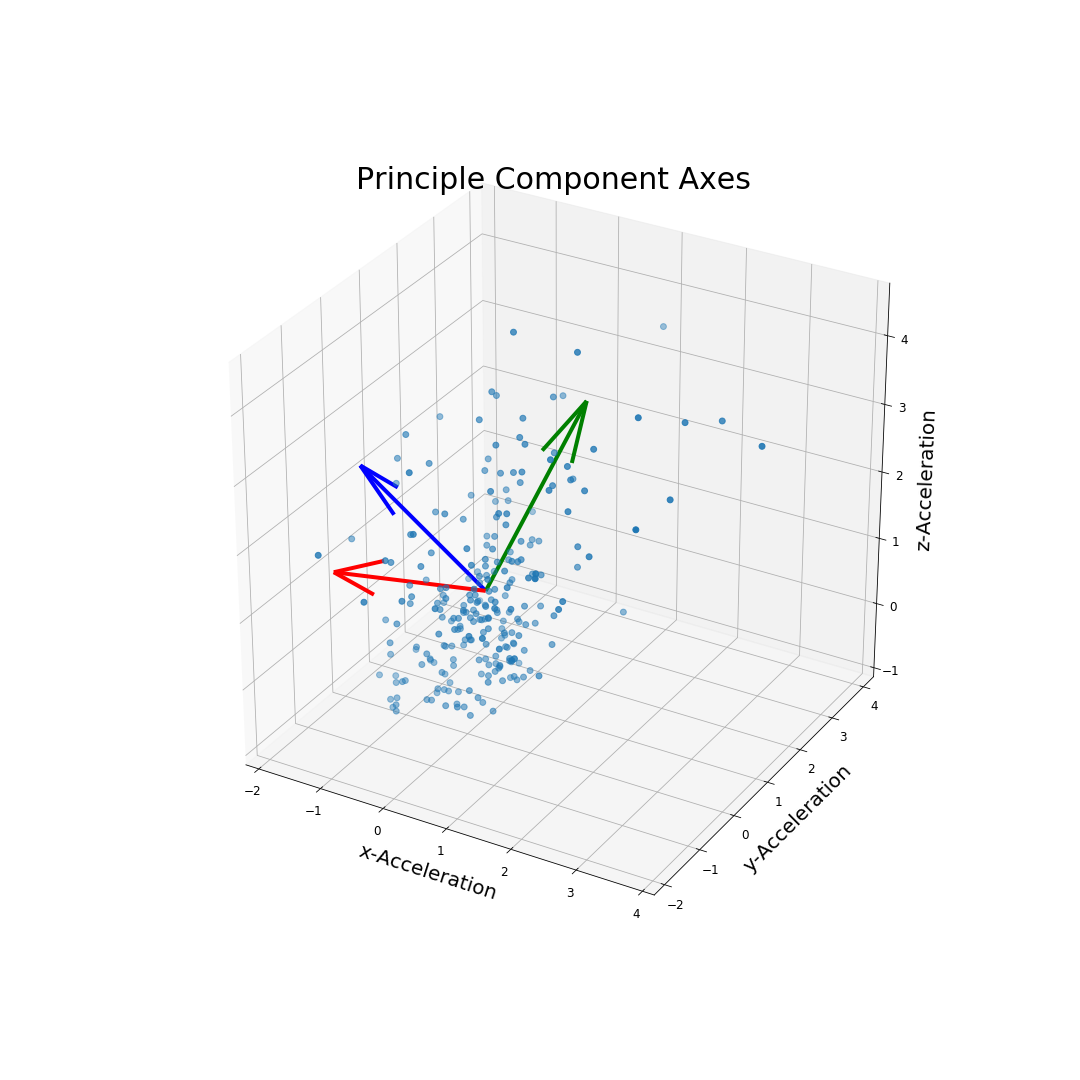
\includegraphics[width=0.8 \textwidth]{images/comparisons/jog_PrincipleAxes.png}
    \caption{The rotated and aligned acceleration data is plotted with the principle axes it has been projected on.}
     \label{fig:alignedPrincipleAxis}
\end{figure}

We rotated each of the acceleration vectors back to their initial positions by using the corresponding orientation measurements, as shown in Eqn.~(\ref{eqn:quaternion_final}) below,
\begin{equation}
\label{eqn:quaternion_final}
    R_q(p)^{-1} = q^{*} \odot p \odot q.
\end{equation}
Once the initial rotation was completed for each acceleration vector, we applied Principle Component Analysis (PCA) on the rotated components within a single feature vector. PCA allows us to find the axes of the data that contain the most variation. We normalize the axes, and then project the data onto the principle axes. Now, most of the variation in the signal will be isolated on the major axis, rather than across multiple axes. This transformation is shown in Fig.~\ref{fig:rotationAlignmentComp}. The principle axes with the projected acceleration data is shown in Fig.~\ref{fig:alignedPrincipleAxis}.


\subsection{Final Dataset Cross Validation}
\label{sub:actual_results}

After processing the acceleration data based on the orientation and PCA rotations, we ran our cross dataset evaluation using the extra-trees and k-NN classifiers. Our results are summarized in Tables~\ref{tab:128_rot}~and~\ref{tab:256_rot} below.

\begin{table}[H]
\centering
\caption{Cross Dataset Rotated Accuracy, 128 Feature Length}
\begin{tabular}{lcl}
\toprule
\multicolumn{1}{l}{\textbf{Test Dataset}} & \multicolumn{1}{c}{\textbf{k-NN}} & \multicolumn{1}{c}{\textbf{Trees}}  \\ \midrule
\textsc{MotionSense} & 28.7\%  & 46.2\% \\
\textsc{MobiAct}     & 34.5\% & 62.6\% \\
\bottomrule
\end{tabular}
\label{tab:128_rot}
\end{table}

\begin{table}[H]
\centering
\caption{Cross Dataset Rotated Accuracy, 256 Feature Length}
\begin{tabular}{lcl}
\toprule
\multicolumn{1}{l}{\textbf{Test Dataset}} & \multicolumn{1}{c}{\textbf{k-NN}} & \multicolumn{1}{c}{\textbf{Trees}}  \\ \midrule
\textsc{MotionSense} & 27.8\% & 46.0\% \\
\textsc{MobiAct}     & 32.2\% & 52.4\% \\
\bottomrule
\end{tabular}
\label{tab:256_rot}
\end{table}

If we compare these results to the results of the na\"ive data analysis that are summarized in Tables~\ref{tab:128naive}~and~\ref{tab:256naive}, then we see that our accuracy actually decreased. There are a few reasons for why this may be the case.

The first reason, we believe, is that there may be an error in our data preprocessing for the \textsc{MobiAct} dataset when we orient the data to the principal components of accelerometer feature vector. Specifically, either the orientation data in unreliable or the description of what the orientation data represents is ambiguous, so by orienting the accelerometer data into the navigational frame, we are actually corrupting the data rather then enhancing it. To test this idea, we tried testing our data on data that has only been rotated to the principal axes of the accelerometer data to the phone's body frame without orienting the accelerometer data by the roll, pitch, and yaw angles. The results of this summarized in Tables~\ref{tab:128_pca}~and~\ref{tab:256_pca} below.

\begin{table}[H]
\centering
\caption{Cross Dataset PCA Accuracy, 128 Feature Length}
\begin{tabular}{lcl}
\toprule
\multicolumn{1}{l}{\textbf{Test Dataset}} & \multicolumn{1}{c}{\textbf{k-NN}} & \multicolumn{1}{c}{\textbf{Trees}}  \\ \midrule
\textsc{MotionSense} & 25.9\%  & 54.5\% \\
\textsc{MobiAct}     & 15.1\% & 48.1\% \\
\bottomrule
\end{tabular}
\label{tab:128_pca}
\end{table}

\begin{table}[H]
\centering
\caption{Cross Dataset PCA Accuracy, 256 Feature Length}
\begin{tabular}{lcl}
\toprule
\multicolumn{1}{l}{\textbf{Test Dataset}} & \multicolumn{1}{c}{\textbf{k-NN}} & \multicolumn{1}{c}{\textbf{Trees}}  \\ \midrule
\textsc{MotionSense} & 23.1\% & 54.7\% \\
\textsc{MobiAct}     & 14.6\% & 53.9\% \\
\bottomrule
\end{tabular}
\label{tab:256_pca}
\end{table}

Notably, these results demonstrate that rotating the data to the accelerometer's principle components also decreases the accuracy of our classifier across datasets. This decrease could be due to a few reasons. First and foremost, for sedentary activities---such as sitting, standing, and laying down---the relative orientation of a smartphone matters. By transforming our data into its principal components, we lose important relative orientation information of the smartphone. When we look at our results more clearly, this is exactly what we find.

In order to isolate the effect of the preprocessing (avoiding differences in the signature of specific activities across datasets), we looked more closely at the performance of the pre-processing on the \textsc{Motion Sense} dataset. Figure~\ref{fig:confusion_mat} illustrates that the classifiers of the raw data does a much better job at accurately distinguishing between sitting and standing. However, after transforming the data to its principle axes, we lose this ability as we have implicitly erased the orientation information that the classifier was was depending on.


\begin{figure}[ht]
\begin{subfigure}{.5\textwidth}
  \centering
  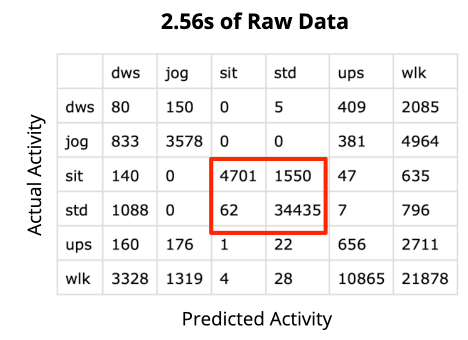
\includegraphics[width = \textwidth]{images/comparisons/conf_raw.png}
   \caption{Raw data.}
     \label{fig:cm-raw}
\end{subfigure}
\begin{subfigure}{.5\textwidth}
  \centering
   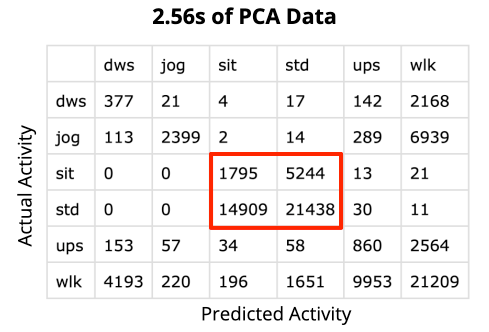
\includegraphics[width = \textwidth]{images/comparisons/conf_pca.png}
    \caption{Data rotate to Principle Axes.}
     \label{fig:cm-pca}
\end{subfigure}
%%
%%
\caption{The confusion matrices for an extra tree classifier trained on the \textsc{Motion Sense} dataset, cross validated by user. The red box highlights the major differences in our activities: by rotating the data to the principal components, our classifier is no longer able to distinguish between the sitting and standing activities as both are relatively sedentary and the only major difference is the phone's orientation.}
\label{fig:confusion_mat}
\end{figure}



\subsubsection{Orientation Visualization}
\label{sub:orien_vis}

Although our idea of rotating the data based on the orientation angles seemed like a promising approach, our initial results in Sec.~\ref{sub:actual_results} were far from what we had hoped. We decided to inspect the orientation angles to make sure that they were reasonably similar for the same activities between datasets, as shown in Fig.~\ref{fig:sitting_Globe}.

\begin{figure}[hb]
\begin{subfigure}{.5\textwidth}
  \centering
    \includegraphics[width = \textwidth]{images/heading/256/mobiAct/sit.png}
    \caption{Mobi Act Dataset}
    \label{fig:mobiAct_sitting_orient}
\end{subfigure}
\begin{subfigure}{.5\textwidth}
  \centering
  % include second image
  \centering
  \includegraphics[width=\linewidth]{images/heading/256/motionSense/sit.png}  
  \caption{Motion Sense Dataset}
  \label{fig:motionSense_sitting_orient}
\end{subfigure}
\caption{The images above are based on the orientation data for a random user in each dataset. There is significant difference in the clustering of the orientation data between the two datasets used.}
\label{fig:sitting_Globe}
\end{figure}

While the Motion Sense dataset had relatively distinct clusters of data, the MobiAct data was much more spread out. We then visualized the orientation angles individually, as shown in Figure~\ref{fig:YPR_comp}. This furthered our suspicion that the given angles for the two datasets had different conventions and/or had different ranges of operation. Unfortunately, there was not any information on either of these crucial components.

\begin{figure}[H]
\begin{subfigure}{.5\textwidth}
  \centering
    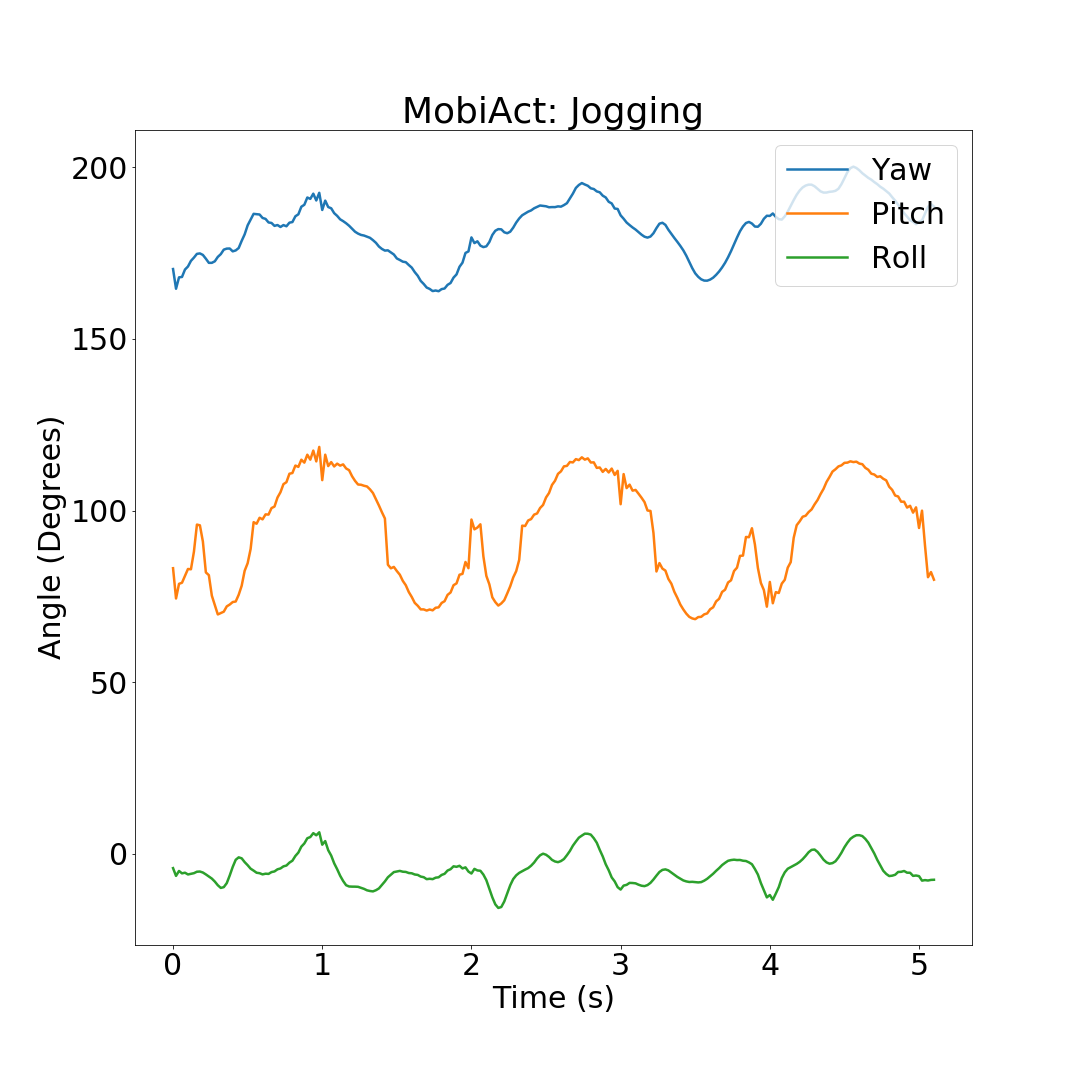
\includegraphics[width = \textwidth]{images/comparisons/mobiActJoggingYPR.png}
    \caption{Mobi Act Dataset}
    \label{fig:mobiAct_YPR}
\end{subfigure}
\begin{subfigure}{.5\textwidth}
  \centering
  % include second image
  \centering
  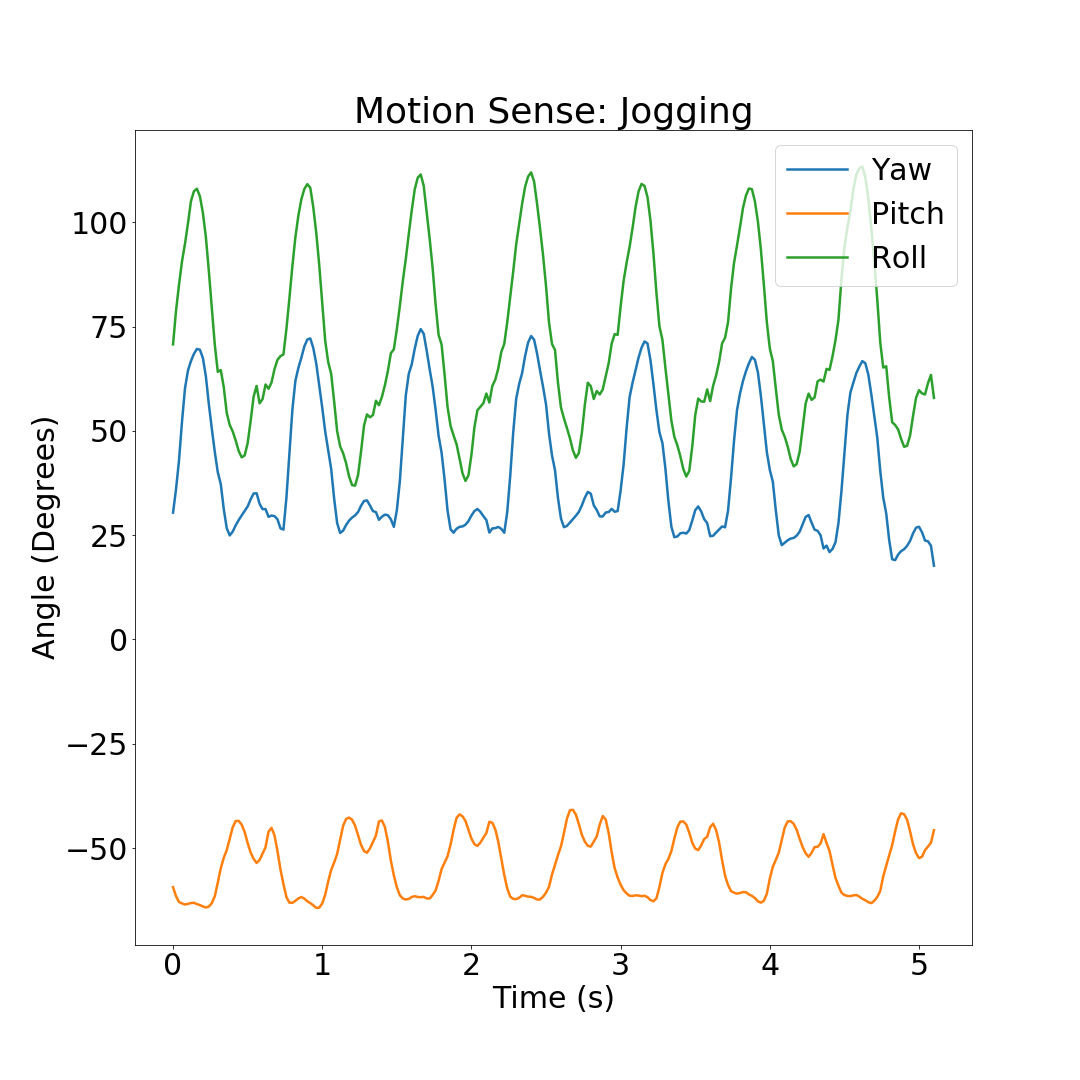
\includegraphics[width=\linewidth]{images/comparisons/motionSenseJoggingYPR.png}  
  \caption{Motion Sense Dataset}
  \label{fig:motionSense_YPR}
\end{subfigure}
\caption{The images above are based on the orientation angles for a random user in each dataset.}
\label{fig:YPR_comp}
\end{figure}

\subsection{Final Verdict on Orientation Processing}

Ultimately, we believe that the orientation processing, as we presented it in this section, introduces more error into our dataset than it is worth. The combination of an ambiguous pitch, roll, and yaw measurements in the dataset with the unpredictability of PCA on our clearly non-linear data gives us pause to continue down this path. However, our goal remains the same: to create orientation and time independent features, in order to create a human activity recognition algorithm that is robust to different orientations of the phone. 

To do this, we plan on using the curvature and torsion of velocity as coordinate invariant representations of the phone's movement. The question still remains whether we need to transform the phone from a body frame to a navigation frame to do this effectively. For these coordinate invariant features, we only consider data from a \SI{0.06}{s} period (3 data points), so we believe that the variation in orientation is small enough that adjusting for orientation is not necessary. Indeed, due to the uncertainties in the orientation data, we believe that this could cause more harm than good.




